\paragraph{QuizziPedia::Back-End::App::Controllers::LangController}
\label{QuizziPedia::Back-End::App::Controllers::UserController}
\begin{figure}[ht]
	\centering
	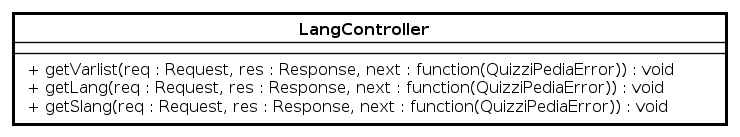
\includegraphics[scale=0.8]{UML/Classi/Back-End/QuizziPedia_Back-End_App_Controllers_langController.png}
	\caption{QuizziPedia::Back-End::App::Controllers::LangController}
\end{figure}
\FloatBarrier
\begin{itemize}
	\item 
	\textbf{Descrizione}:
	classe che gestisce la logica applicativa riguardante il passaggio della traduzione delle variabili;
	\item \textbf{Utilizzo}:
	viene utilizzata per gestire la richiesta di traduzione delle variabili;
	\item \textbf{Relazioni con altre classi}:
	\begin{itemize}
		\item \textbf{IN LangModel}: classe che modella le informazioni riguardanti la lingua dell'applicazione.
	\end{itemize}
	\item \textbf{Metodi}:
		\begin{itemize}
			\item \texttt{+ getVarlist(req: Request, res: Response,\\ next: function(QuizziPediaError)): void} \\
			Ritorna la lista di variabili con la loro traduzione.
			\textbf{Parametri}:
				\begin{itemize}
					\item \texttt{req: Request} \\
					Rappresenta la richiesta inviata al server\ped{G}. Contiene la stringa che indica la lingua che si vuole tradurre le variabili;
					\item \texttt{res: Response} \\
					Rappresenta la risposta che il server fornirà al termine  dell'esecuzione del metodo;
					\item \texttt{next: function(QuizziPediaError)} \\
					Rappresenta la \textit{callback\ped{G}} che il metodo deve chiamare al termine dell'elaborazione per passare il controllo ai successivi \textit{middleware\ped{G}}. La presenza del parametro facoltativo \textit{QuizziPediaError} attiva la catena di gestione dell'errore in sostituzione della normale catena di gestione delle richieste.
				\end{itemize}
				\item \texttt{+ getLang(req: Request, res: Response,\\ next: function(QuizziPediaError)): void} \\
				Ritorna un array di stringhe contenenti le lingue usate nell'applicazione. 
			\textbf{Parametri}:
				\begin{itemize}
					\item \texttt{req: Request} \\
					Rappresenta la richiesta inviata al server\ped{G};
					\item \texttt{res: Response} \\
					Rappresenta la risposta che il server fornirà al termine  dell'esecuzione del metodo;
					\item \texttt{next: function(QuizziPediaError)} \\
					Rappresenta la \textit{callback\ped{G}} che il metodo deve chiamare al termine dell'elaborazione per passare il controllo ai successivi \textit{middleware\ped{G}}. La presenza del parametro facoltativo \textit{QuizziPediaError} attiva la catena di gestione dell'errore in sostituzione della normale catena di gestione delle richieste.
				\end{itemize}
				\item \texttt{+ getSlang(req: Request, res: Response,\\ next: function(QuizziPediaError)): void} \\
				Ritorna un'abbreviazione della lingua usata nell'applicazione.
			\textbf{Parametri}:
				\begin{itemize}
					\item \texttt{req: Request} \\
					Rappresenta la richiesta inviata al server\ped{G}.
					\item \texttt{res: Response} \\
					Rappresenta la risposta che il server fornirà al termine  dell'esecuzione del metodo;
					\item \texttt{next: function(QuizziPediaError)} \\
					Rappresenta la \textit{callback\ped{G}} che il metodo deve chiamare al termine dell'elaborazione per passare il controllo ai successivi \textit{middleware\ped{G}}. La presenza del parametro facoltativo \textit{QuizziPediaError} attiva la catena di gestione dell'errore in sostituzione della normale catena di gestione delle richieste.
				\end{itemize}
		\end{itemize}
\end{itemize}
